% !TeX encoding = UTF-8
% !TeX program = xelatex
% !TeX spellcheck = fr
% !TeX root = tm_astro_main.tex


	
\chapter{Evolution stellaire}\label{2}

\section{La séquence principale}\label{2.1}

Lorsqu’une étoile s’est formée, des réactions nucléaires commencent à s’amorcer dans son cœur sous l’effet de la pression engendrée par la force gravitationnelle. Ces réactions qui peuvent durer plusieurs milliards d’années consistent principalement à fusionner de l’hydrogène en hélium. Il existe deux processus pour arriver à cela : la chaîne proton-proton et le cycle Carbone-Azote-Oxygène.

\subsection{La chaîne proton-proton}\label{2.1.1}


\begin{equation}\ce{\ce{1H} + \ce{1H} -> \ce{2D} + \ce{e+} + $\nu_{e}$}\label{Eq. 2.1}\end{equation}
\begin{equation}\ce{\ce{2D} + \ce{1H} -> \ce{3He} + g}\label{Eq. 2.2}\end{equation}
\begin{equation}\ce{\ce{3He} + \ce{3He} -> \ce{4He} + \ce{21H}}\label{Eq. 2.3}\end{equation}\smallskip	


La fusion de l’hydrogène ne fait pas que de produire de l’hélium, elle libère aussi beaucoup d’énergie. Ce processus crée une pression qui est capable de compenser la compression gravitationnelle et ainsi permet d’équilibrer thermodynamiquement l’étoile (§\ref{1}).
Nous pouvons expliquer la longévité de cette phase de vie d’une étoile par la lenteur de la réaction (Eq. \ref{Eq. 2.1}). En effet, l’Eq. \ref{Eq. 2.1} décrit une interaction faible qui est par définition extrêmement lente à cause de sa faible section efficace (probabilité qu’une interaction de type faible se produise).

\subsection{Le cycle CNO}\label{2.1.2}

Les étoiles composées de gaz enrichis de plusieurs générations stellaires possèdent déjà des éléments lourds comme le carbone, l’azote ou bien encore l’oxygène dans leur composition. Ces éléments servent de très bons catalyseurs pour créer de l’hélium.


\begin{equation}\ce{\ce{12C} + \ce{1H} -> \ce{13N} +$\gamma$}\label{Eq. 2.4}\end{equation}				     	
\begin{equation}\ce{\ce{13N} -> \ce{13C} + \ce{e+} + $\nu_{e}$ }\label{Eq. 2.5}\end{equation}					   	
\begin{equation}\ce{\ce{13C} + \ce{1H} -> \ce{14N} + $\gamma$ }\label{Eq. 2.6}\end{equation}	
\begin{equation}\ce{\ce{14N} + \ce{1H} -> \ce{15O} + $\gamma$}\label{Eq. 2.7}\end{equation}\newpage\vspace{2cm}		
\begin{equation}\ce{\ce{15O} -> \ce{15N} + \ce{e+} + $\nu_{e}$	}\label{Eq. 2.8}\end{equation}
\begin{equation}\ce{\ce{15N} + \ce{1H} -> \ce{12C} + \ce{4He}}\label{Eq. 2.9}\end{equation}\smallskip

\begin{figure}[H]
	\centering
	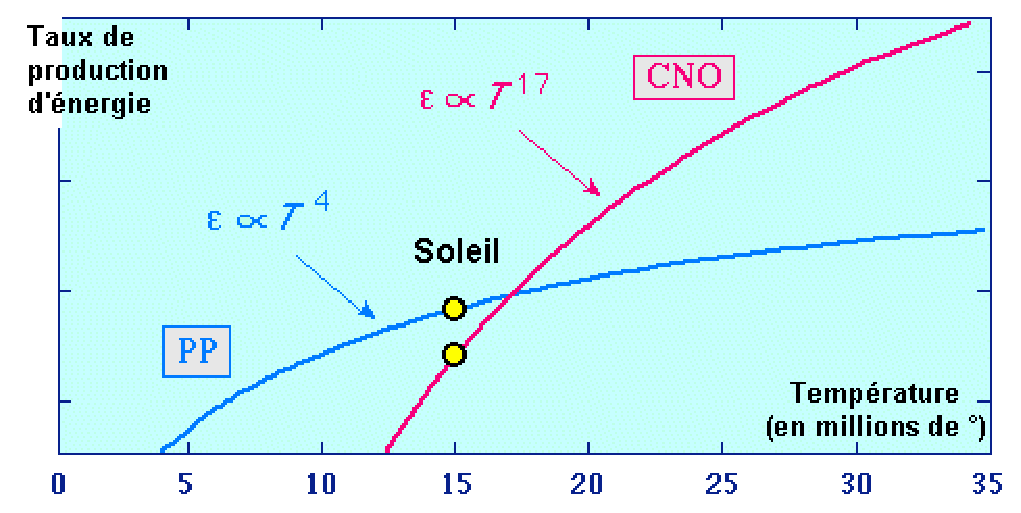
\includegraphics[scale=0.8]{images/cno-pp}
	\caption[Comparaison des cycles PP et CNO\newline\url{http://nrumiano.free.fr/Fetoiles/energie.html}]{Comparaison des cycles PP et CNO}
	\label{Fig. 2.1}
\end{figure}\bigskip

Le graphique ci-dessus nous montre que la chaîne proton-proton reste la principale source d’énergie des étoiles allant jusqu’à 2 $M_\odot$. Dans les étoiles de ce type, l’énergie est transmise de manière radiative dans le cœur, tandis que dans les couches supérieures, c’est la convection qui la transporte. Lorsque les 2 $M_\odot$ sont dépassées, le cycle CNO devient plus fréquent que la chaîne proton-proton. Cette limite franchie, les couches intérieures de l’étoile reçoivent leur énergie plutôt de manière convective, alors que les couches supérieures la reçoive par radiation.

\subsection{Le diagramme de Hertzsprung-Russell}\label{2.1.3}

Même si toutes les étoiles sont soumises à ces cycles de production de l’hélium, elles ne sont pas toutes les mêmes. Elles se distinguent notamment par des différences de luminosité, de types spectrales (couleurs) ou bien encore de masse. Ce diagramme (Fig. \ref{Fig. 2.2}), nommé d’après ses créateurs, représente des populations d’étoiles classées selon leur luminosité et leur type spectrale. La masse n’est pas représentée comme l’un des axes car elle est étroitement liée à la luminosité de l’étoile (Eq. \ref{Eq. 2.10}).

\begin{center}
\begin{equation}L \propto M^{3}\label{Eq. 2.10}\end{equation}
\end{center}\newpage

\begin{figure}[H]\vspace{1cm}
	\centering
	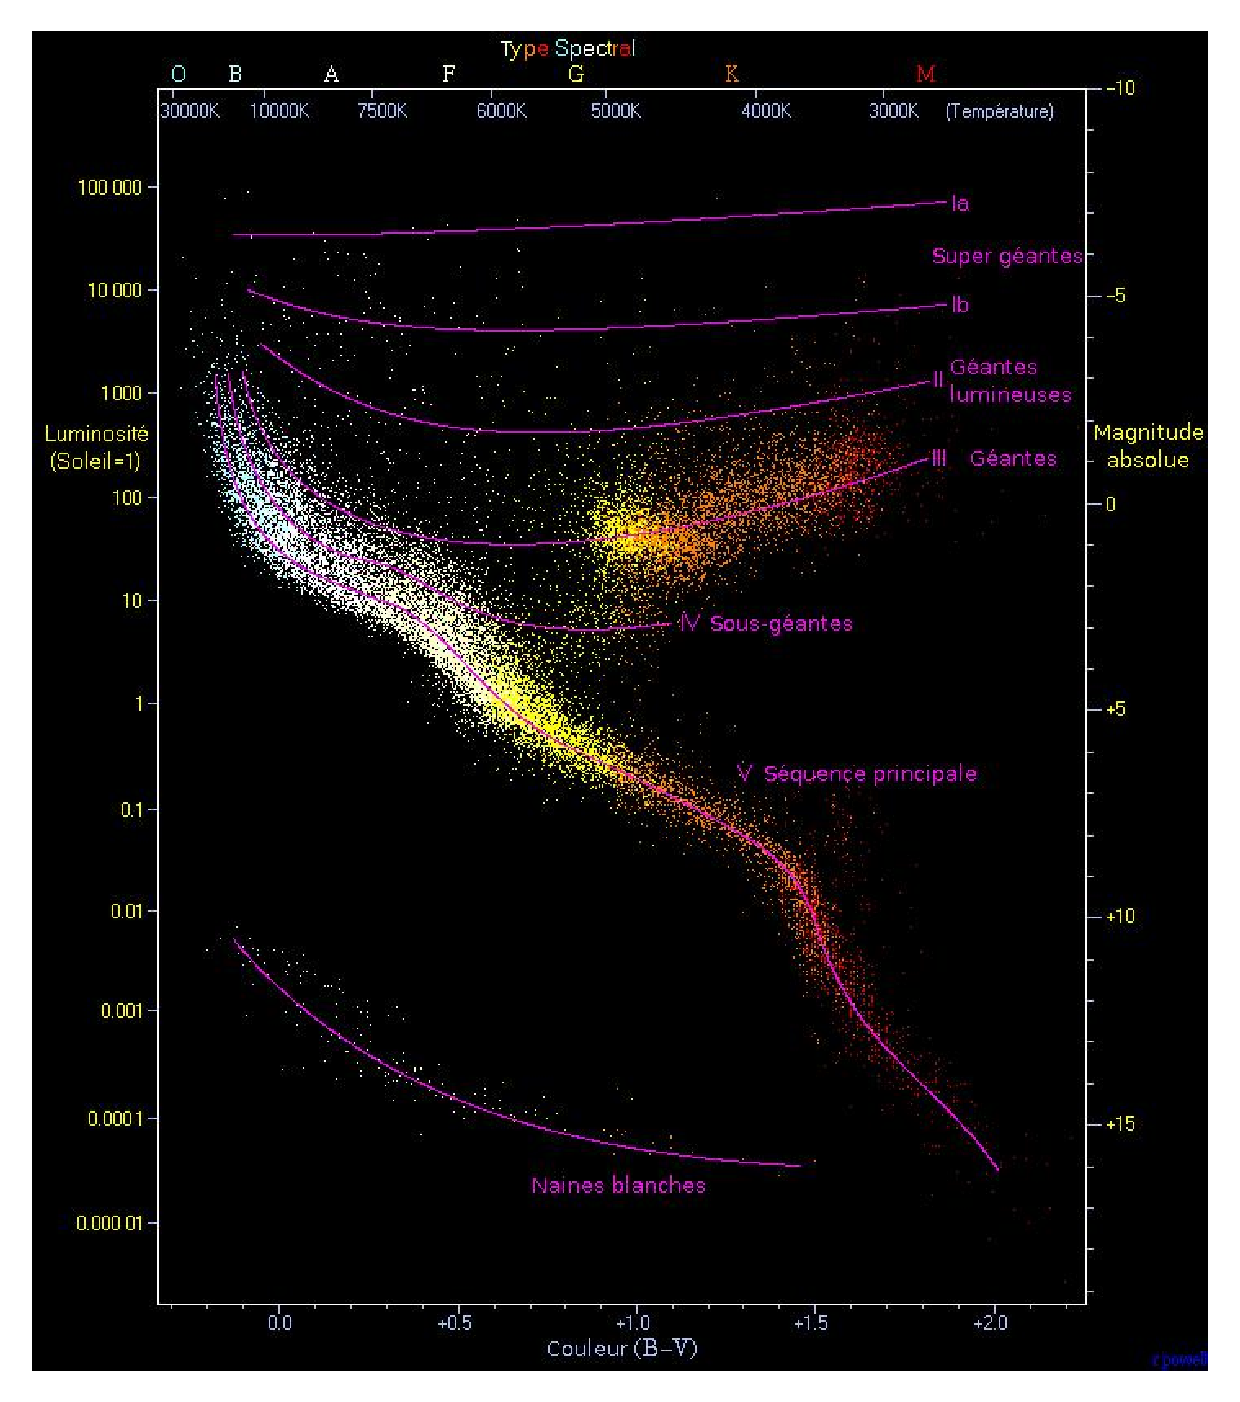
\includegraphics[scale=0.4]{images/hr-diagram}
	\caption[Diagramme de Hertzsprung-Russell\newline\url{http://www.astrosurf.com/luxorion/vie-etoiles2.html}]{Diagramme de Hertzsprung-Russell}
	\label{Fig. 2.2}
\end{figure}\bigskip

Nous pouvons facilement distinguer que certaines zones bien précises se délimitent, elles représentent les différents types d’étoiles. De plus, tout au long de sa vie une étoile se déplace dans ce diagramme. Par exemple, le soleil achèvera son existence dans la branche des naines blanches. Le diagramme HR représente l’un des outils les plus importants de l’astrophysique moderne, car il permet de prédire l’emplacement d’une étoile et en suite de le comparer avec les observations effectuées sur ce même objet.\bigskip

\section{La phase géante rouge}\label{2.2}

Les réserves d’hydrogène d’une étoile ne sont pas illimitées. En effet, il arrive un moment où il n’y a plus assez d’hydrogène dans le cœur de l’étoile pour entretenir les fusions nucléaires, la pression engendrée par ces réactions disparaît et donc l’équilibre hydrostatique est rompu. Le cœur, alors principalement composé d’hélium, ne possède pas la température nécessaire pour débuter la fusion de l’hélium ($10^{8}$ K), il se contracte alors à cause de la pression gravitationnelle. Sous l’effet de cette contraction, l’enveloppe d’hydrogène entourant le noyau atteint une température suffisante pour réamorcer la fusion nucléaire. L’agrandissement du rayon de l’étoile s’explique de deux manières différentes :

\begin{figure}[H]\vspace{1cm}
	\centering
	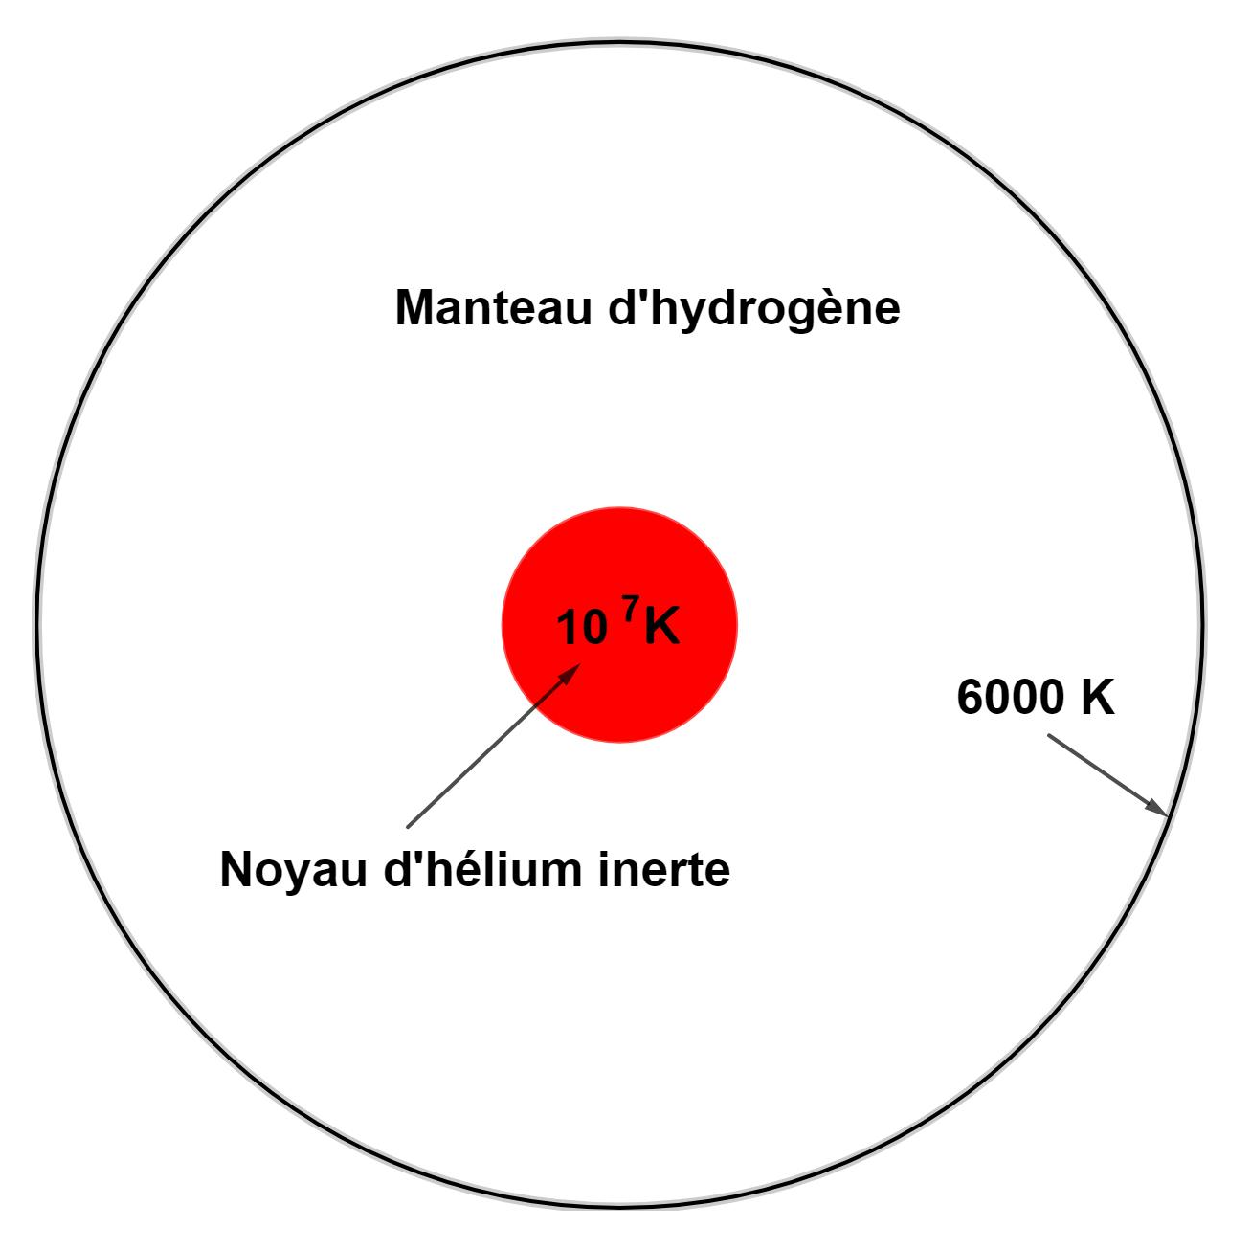
\includegraphics[scale=0.45]{images/compo_sp}
	\caption[Composition d'une étoile (soleil) à la fin de la séquence principale -figure réalisée avec GeoGebra]{Composition d'une étoile (soleil) à la fin de la séquence principale}
	\label{Fig. 2.3}
\end{figure}\bigskip                         

\begin{enumerate}
	\item L’énergie produite par la fusion en couche de l’hydrogène réchauffe et donc dilate l’enveloppe stellaire.
	\item La contraction du noyau de l’étoile est stoppée par la pression de dégénérescence des électrons (annexe). Cette pression d’origine quantique découle tout droit du principe d’exclusion de Pauli (deux électrons ne peuvent pas se trouver dans le même état quantique). Autrement dit, il existe une pression limite que nous ne pouvons pas franchir car toutes les couches électroniques de basses énergies d’un atome sont occupées. Lorsque cette limite est atteinte, l’énergie associée à la compression gravitationnelle se transforme en énergie thermique. La température du cœur va alors augmenter drastiquement, sans que pour autant la pression ne varie, et ainsi dilater les couches extérieures de l’étoile qui, elles, vont diminuer de température, d’où la couleur rouge, orange qui correspond à une plus faible température. 
	
\end{enumerate}

\subsection{Flash de l'hélium}\label{2.2.1}

Pour les étoiles comprises entre 0,5 et 2 $M_\odot$, il existe un phénomène extrêmement puissant qui se produit lorsque le cœur de l’étoile atteint les $10^{8}$ K, température nécessaire pour amorcer la fusion de l’hélium. En quelques instants, tout le noyau de l’étoile enclenche la fusion de l’hélium en carbone (réaction triple alpha). Cette explosion génère autant de luminosité que toute une galaxie, cependant la majorité de cette énergie est absorbée par le plasma de l’étoile qui se dilate fortement. Lorsque l’énergie thermique du noyau redevient inférieure à l’énergie de Fermi, son gaz n’est plus dégénéré. L’étoile se retrouve donc sur une sorte de nouvelle séquence principale (en plus court), mais cette fois-ci elle fusionne de l’hélium pour former du carbone et de l’oxygène en son centre. De plus, l’enveloppe d’hydrogène qui entoure le noyau continue aussi à former de l’hélium.\smallskip

Quant aux étoiles supérieures à 2 $M_\odot$, elles sont suffisamment massives pour atteindre les conditions requises à la réaction triple alpha sans passer par les flashs de l’hélium.\newpage

\begin{figure}[H]\vspace{1cm}
	\centering
	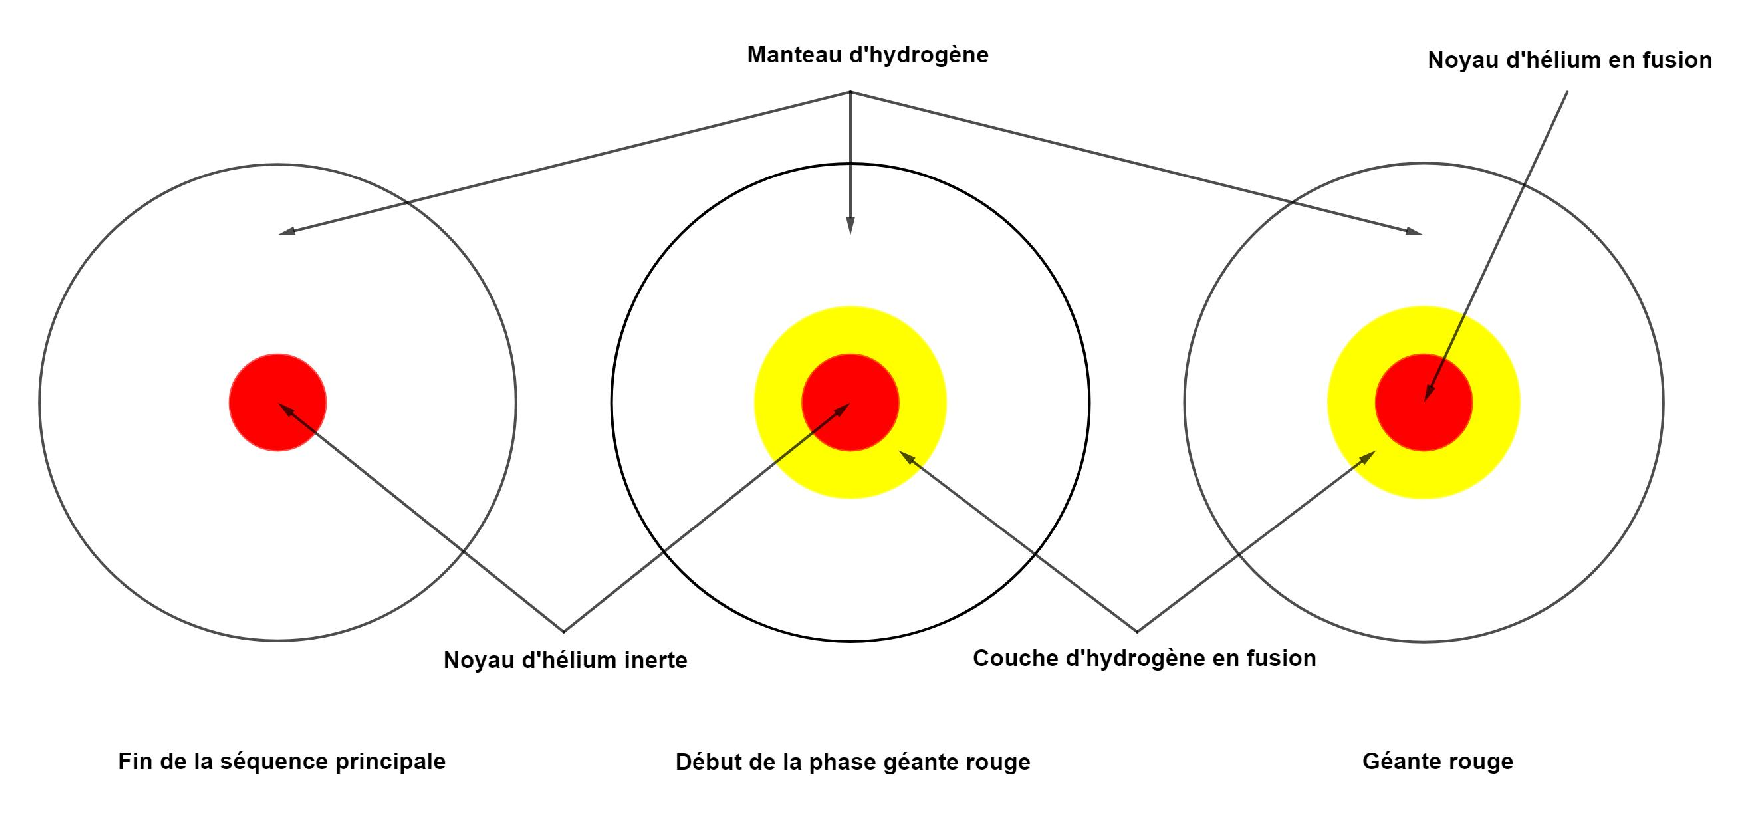
\includegraphics[scale=0.40]{images/compo_sp_gr}
	\caption[Comparaison entre les différentes premières phases de fusion d'une étoile (pas à l'échelle) - figure réalisée avec GeoGebra]{Comparaison entre les différentes premières phases de fusion d'une étoile (pas à l'échelle)}
	\label{Fig. 2.4}
\end{figure}

\subsection{AGB (branche asymptotique des géantes)}\label{2.2.2}

Une fois l’hélium épuisé dans le noyau stellaire le cycle recommence : contraction du cœur, augmentation de la température, reprise des fusions thermonucléaires dans les coquilles d’hydrogène ainsi que d’hélium. La fusion en couche de l’hydrogène et de l’hélium se révèle être très agitée. Ces couches deviennent par moment instables et créent des pulsations thermiques. Ces pulsations ont pour effet de créer des vents stellaires qui font perdre de la masse à l’étoile.

\section{Les naines blanches}\label{2.3}

Les étoiles sont sujettes à expulser d’énormes quantités de masses à cause des vents stellaires. Les étoiles, allant jusqu’à 9 $M_\odot$, se retrouvent avec des masses situées entre 0,6 et 1,1 $M_\odot$ sous l’effet de ces vents. Ces étoiles sont destinées à devenir des naines blanches car elles se trouvent en-dessous de la masse de Chandrasekhar (1,44 $M_\odot$) (annexe). La matière est éjectée de l’étoile de manière symétrique, ainsi se forme une enveloppe, appelée circumstellaire, tout autour du centre de l’étoile. Il ne reste donc plus que le noyau de l’étoile composé d’oxygène et de carbone. Du fait de l’arrêt des réactions thermodynamiques, le centre se contracte jusqu’à ce qu’il s’équilibre une nouvelle fois grâce à la pression de dégénérescence des électrons. Le rayon moyen des naines blanches correspond plus ou moins à celui de la Terre. Cependant, elles possèdent une masse similaire à celle du Soleil, qui possède un rayon 109 fois supérieur à celui de la Terre (Fig. \ref{Fig. 2.3}). De plus, l’enveloppe circumstellaire est illuminée pendant des milliards d’année par la naine blanche en son sein qui se refroidit gentiment, on appelle cela une nébuleuse planétaire. Ces nébuleuses n’ont rien à voir avec des planètes, elles sont historiquement nommées ainsi du fait de leur apparence qui peut faire penser à une planète.\newpage 

\begin{figure}[H]\vspace{1cm}
	\centering
	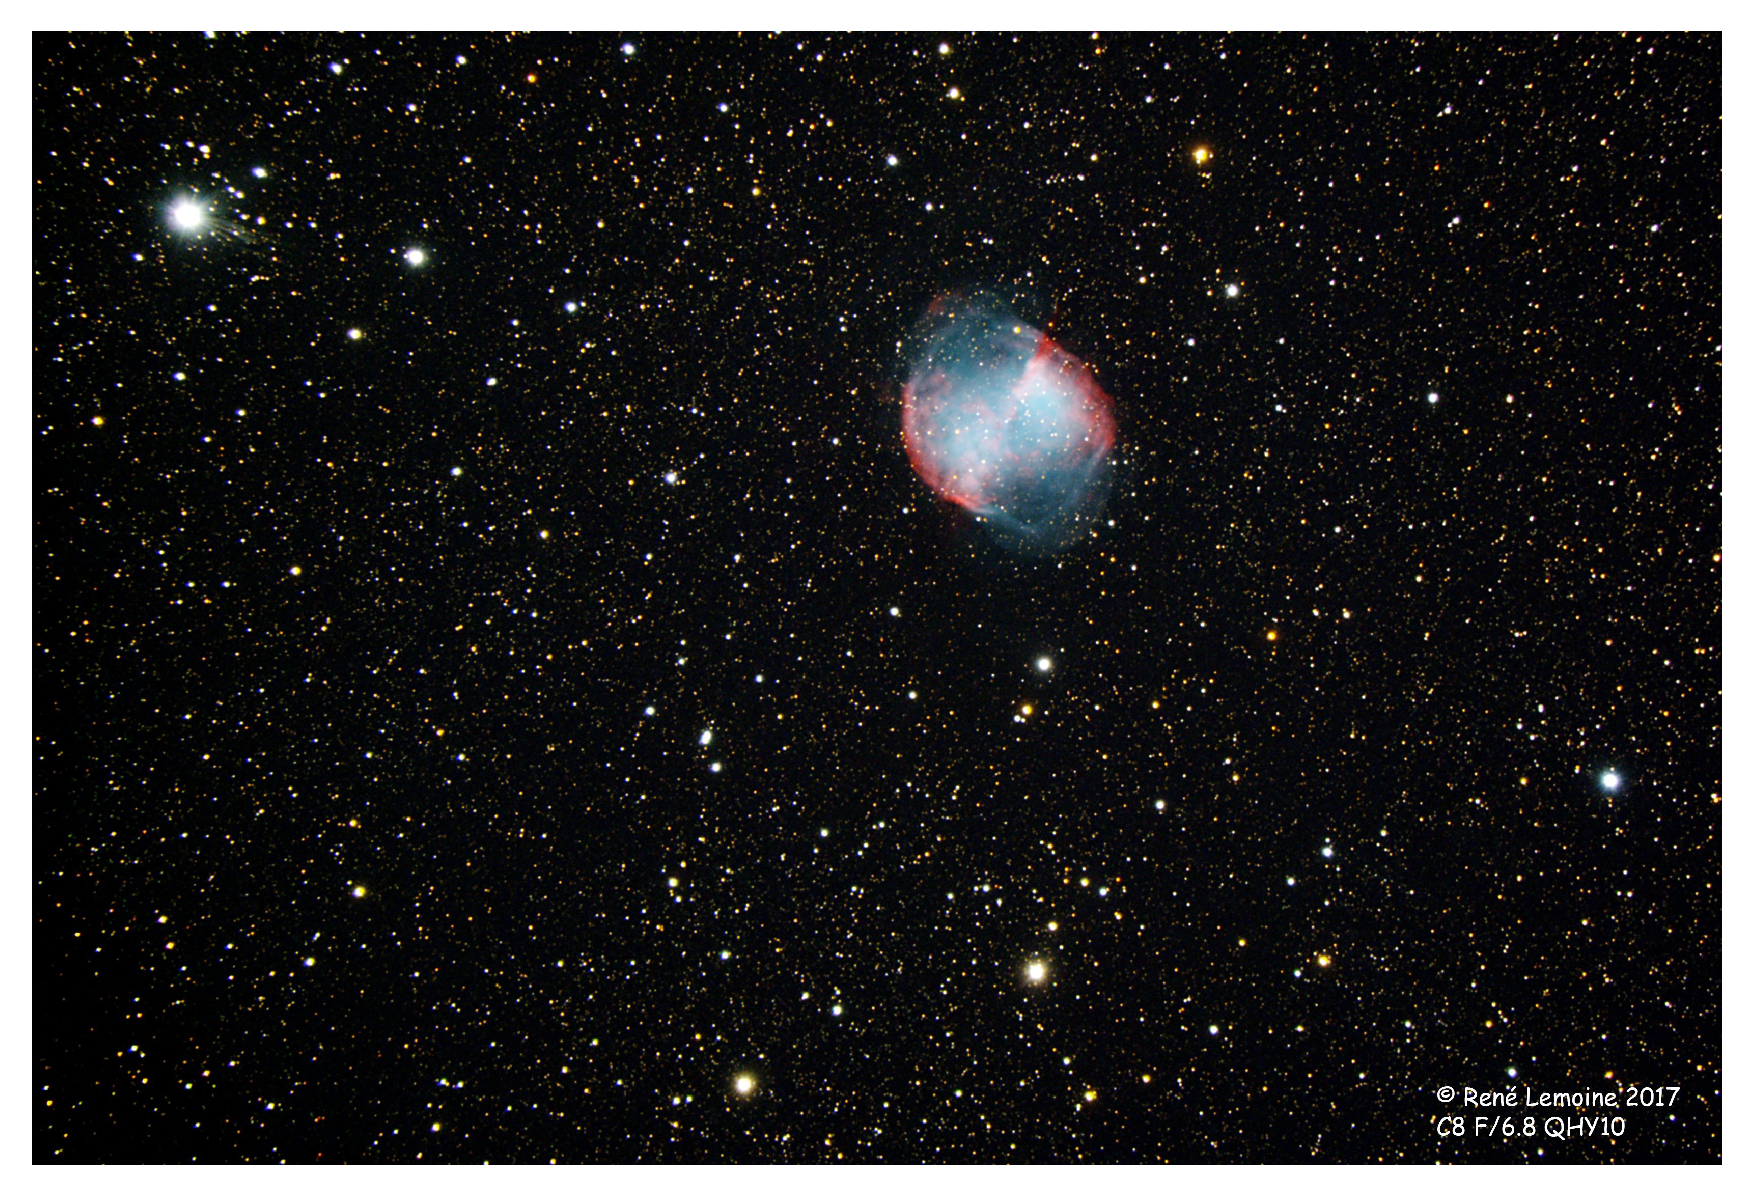
\includegraphics[scale=0.4]{images/m27}
	\caption[M27, nébuleuse planétaire de l'haltère - astrophoto prise par René Lemoine le 30 juillet 2017 avec un Celestron 8 (1h50 de pose)]{M27, nébuleuse planétaire de l'haltère}
	\label{Fig. 2.5}
\end{figure}  

\section{Evolution tardive des étoiles massives}\label{2.4}

Les étoiles de plus de 9 $M_\odot$ ne s’arrêtent pas à la fusion de l’oxygène et du carbone. En effet, leur grande masse leurs permettent d’atteindre de plus grandes échelles de pressions et de températures, ce qui leur permettent de produire des éléments plus lourds comme le magnésium, le néon, le souffre, le silicium ou bien encore le fer. Ces atomes sont produits de manière analogue au carbone et à l’oxygène mais avec des réactions plus complexes. Une des principales caractéristiques de ces étoiles massive est que leur gaz n’est jamais dégénéré (soumis à la pression de dégénérescence des électrons) jusqu’à leur dernier stade d’évolution, lorsque le noyau est constitué de fer. La nucléosynthèse par fusion s’arrête obligatoirement au fer. En effet, le rendement énergétique des réactions de fusion décroit lorsque la masse de l’atome augmente, et c’est à partir de l’élément fer que ces réactions de fusions qui étaient exothermiques, deviennent endothermiques. A ce stade, on dit que l’étoile, appelée supergéante, possède une structure en pelures d’oignon (Fig. \ref{Fig. 2.6}).

\begin{figure}[H]
	\centering
	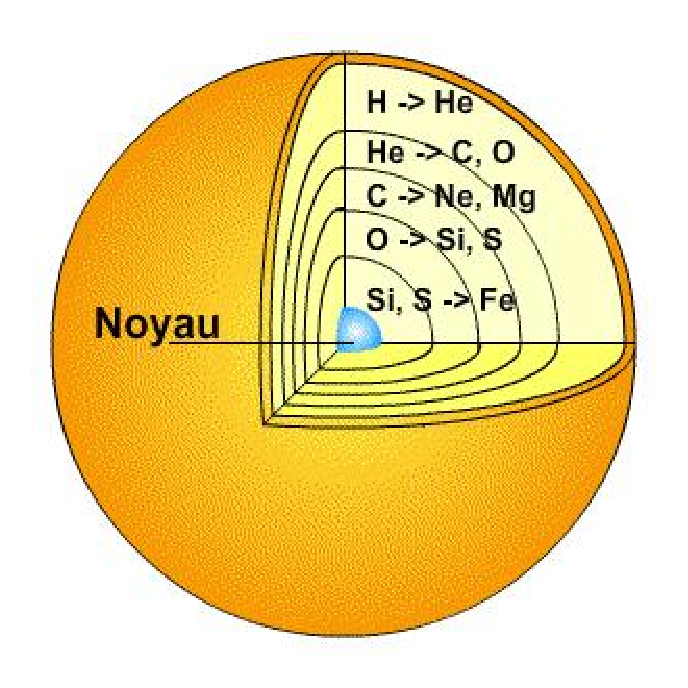
\includegraphics[scale=0.3]{images/oignon}
	\caption[Structure en pelures d'oignon d'une supergéante\newline \url{https://media4.obspm.fr/public/ressources\_lu/pages\_vie-mort/impression.html}]{Structure en pelures d'oignon d'une supergéante}
	\label{Fig. 2.6}
\end{figure}\newpage

Lorsque les réactions thermonucléaires prennent fin dans le cœur de l’étoile, ce dernier se contracte brutalement. Même la pression de dégénérescence des électrons ne suffit pas à compenser la pression gravitationnelle. Les protons capturent les électrons pour ne former plus que des neutrons. Cet effondrement, qui ne dure que quelques secondes, produit une onde de choc pulvérisant la supergéante. Ce phénomène est désigné par le terme de supernova de type II (§\ref{3.1.1}). Il ne reste de cette explosion que le cœur composé de fer. En fonction de sa masse, il deviendra soit une étoile à neutrons soit un trou noir. De plus, toute la matière éjectée forme ce qu’on l’on appelle, le rémanent de la supernova. Les différents types des supernovas seront plus détaillés au chapitre 3 (§\ref{3}).

\begin{figure}[H]
	\centering
	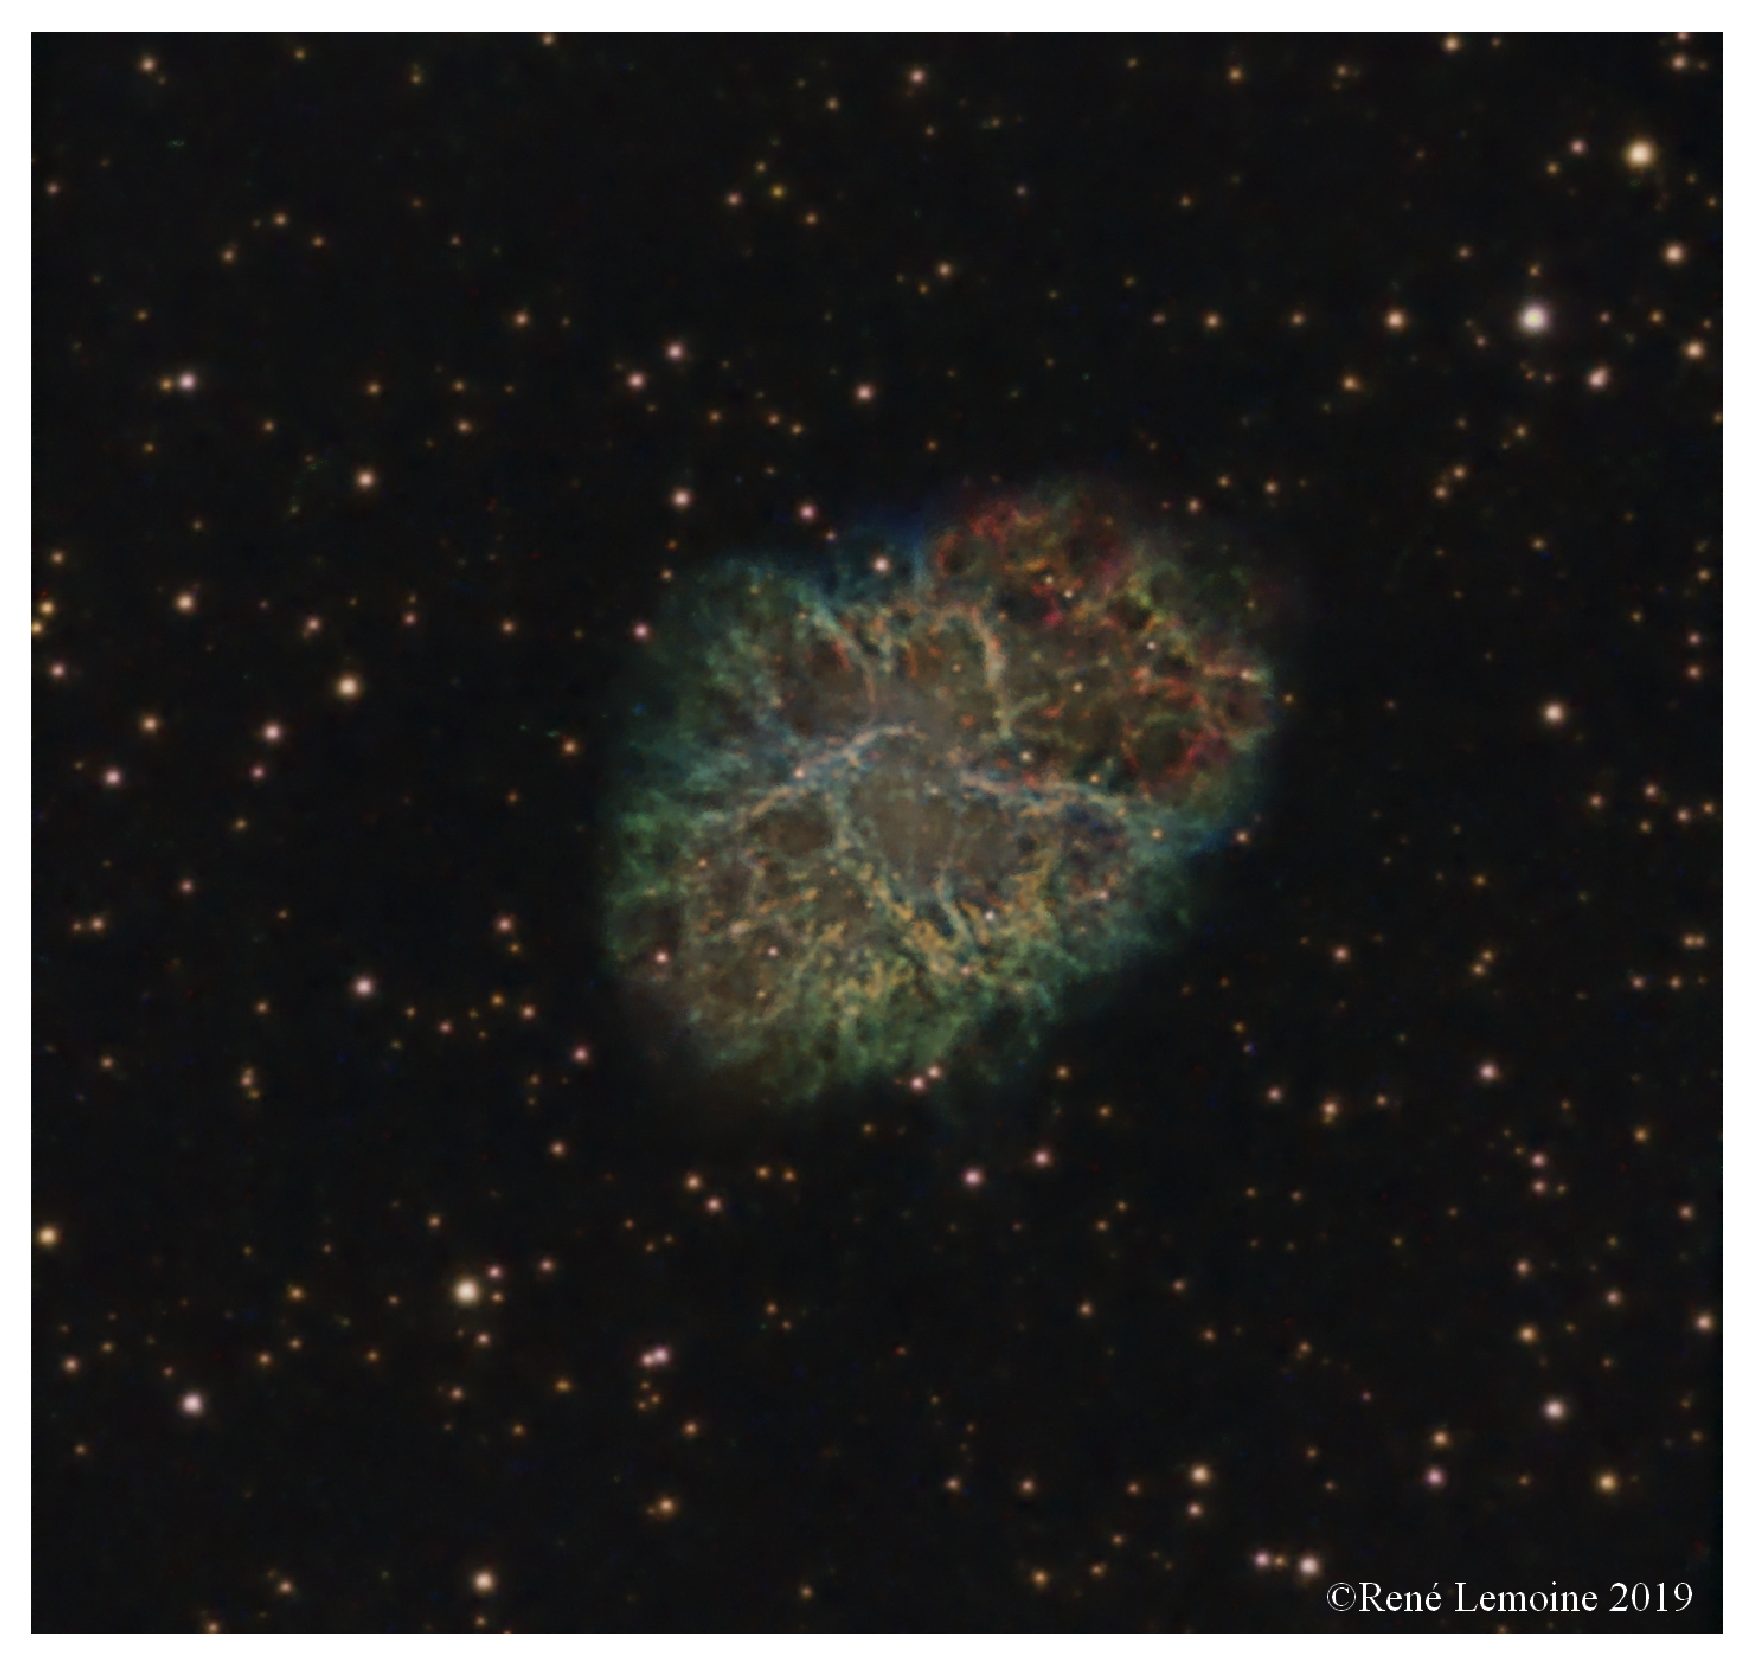
\includegraphics[scale=0.3]{images/m1}
	\caption[M1, nébuleuse du Crabe - astrophoto prise par René Lemoine le 29 janvier 2019 avec un Celestron 8 (6h de pose)]{M1, nébuleuse du Crabe, rémanent d'une supernova datant de 1054}
	\label{Fig. 2.7}
\end{figure}

A titre de comparaison, la nébuleuse de la Fig. \ref{Fig. 2.5} s'étend sur 1,44 années-lumière, tandis que le rémanent de supernova de la Fig. \ref{Fig. 2.7} mesure 5,5 années-lumière. Ces tailles démesurées témoignent de la violence de la mort d'une étoile, que ce soit par explosion en nébuleuse planétaire (§\ref{2.3}) ou par supernova (§\ref{3}). 

\section{Tableau récapitulatif de la nucléosynthèse stellaire}\label{2.5}


